\documentclass{article}
\usepackage{pgfplots}
\pgfplotsset{compat=1.18, width=11cm}

\begin{document}

\begin{figure}[h]
\centering
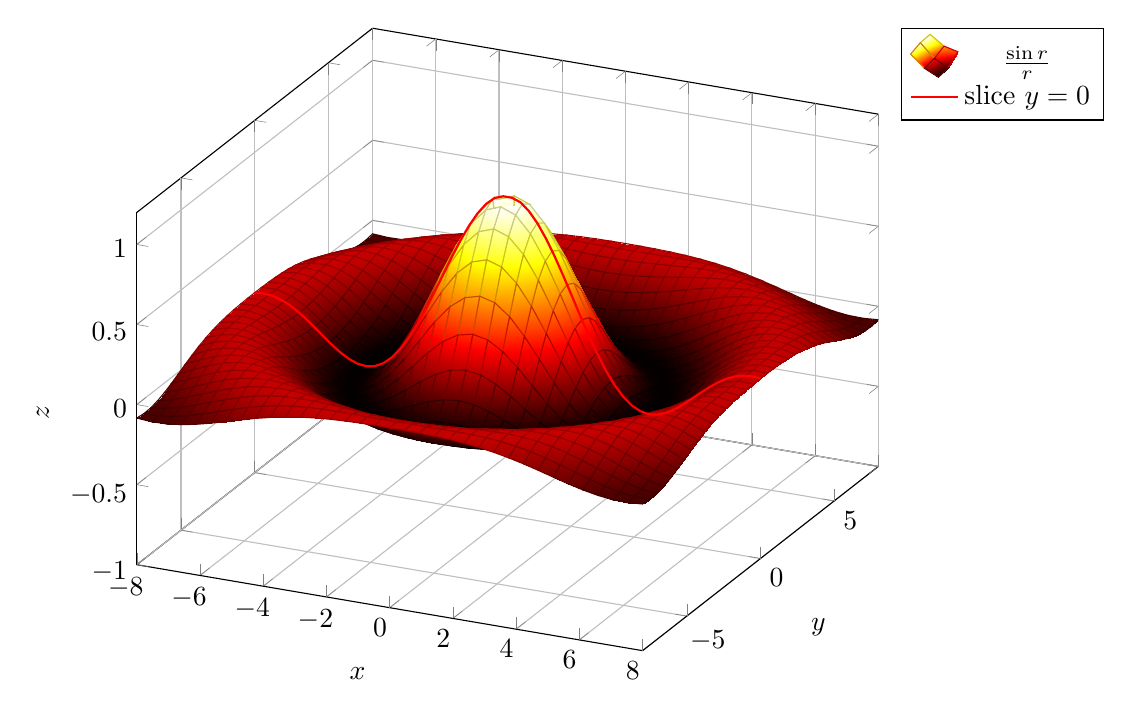
\begin{tikzpicture}
\begin{axis}[
    xlabel={$x$},
    ylabel={$y$},
    zlabel={$z$},
    zmin=-1, zmax=1.2,
    grid=major,
    colormap/hot2,
    legend pos=outer north east,
]
\addplot3[surf, shader=faceted interp, samples=35, domain=-8:8] {sin(deg(sqrt(x^2+y^2)))/(sqrt(x^2+y^2)+0.001)};
\addlegendentry{$\frac{\sin r}{r}$}
\addplot3[red, thick, samples=60, samples y=0, domain=-8:8] (x, 0, {sin(deg(abs(x)))/(abs(x)+0.001)});
\addlegendentry{slice $y=0$}
\end{axis}
\end{tikzpicture}
\caption{The sombrero function with its $y=0$ cross-section.}
\end{figure}

\end{document}
